% !TeX program = xelatex
% Сборка всех лекций: python scripts/build_lectures.py из корня репозитория.
\documentclass[aspectratio=169,12pt]{beamer}
\PassOptionsToPackage{no-math}{fontspec}
% Общая преамбула лекций курса. Подключается после \documentclass:
%
%     \documentclass[aspectratio=169,12pt]{beamer}
%     % Общая преамбула лекций курса. Подключается после \documentclass:
%
%     \documentclass[aspectratio=169,12pt]{beamer}
%     % Общая преамбула лекций курса. Подключается после \documentclass:
%
%     \documentclass[aspectratio=169,12pt]{beamer}
%     \input{mlg_preamble}
%
% Здесь только оформление и макросы — ни \title, ни текста слайдов, чтобы
% все презентации курса выглядели одинаково и правились в одном месте.
%
\usepackage{fontspec}
\usepackage{polyglossia}
\setmainlanguage{russian}
\setotherlanguage{english}
% Без Calibri и Consolas (macOS, Linux) берутся шрифты из TeX Live: Carlito
% совпадает с Calibri по ширине знаков, поэтому переносы и раскладка слайдов
% те же; DejaVu Sans Mono уменьшен так, чтобы ширина знака была как у Consolas.
\IfFontExistsTF{Calibri}{%
  \setmainfont{Calibri}
  \setsansfont{Calibri}
}{%
  \setmainfont{Carlito}[Extension=.ttf, UprightFont=*-Regular, BoldFont=*-Bold,
                        ItalicFont=*-Italic, BoldItalicFont=*-BoldItalic]
  \setsansfont{Carlito}[Extension=.ttf, UprightFont=*-Regular, BoldFont=*-Bold,
                        ItalicFont=*-Italic, BoldItalicFont=*-BoldItalic]
}
\IfFontExistsTF{Consolas}{%
  \setmonofont{Consolas}[Scale=0.92]
}{%
  \setmonofont{DejaVuSansMono}[Extension=.ttf, UprightFont=*, BoldFont=*-Bold,
                               ItalicFont=*-Oblique, BoldItalicFont=*-BoldOblique,
                               Scale=0.84]
}

\usepackage{graphicx}
\usepackage{booktabs}
\usepackage{array}

% ---------------------------------------------------------------- оформление
\definecolor{ink}{HTML}{1B2433}
\definecolor{navy}{HTML}{2B4C6F}
\definecolor{brick}{HTML}{B03A2B}
\definecolor{moss}{HTML}{3E7D5A}
\definecolor{plum}{HTML}{6B5B95}
\definecolor{ash}{HTML}{8B9299}
\definecolor{paper}{HTML}{ECEFF3}

\usetheme{default}
\usecolortheme{default}
\setbeamercolor{structure}{fg=navy}
\setbeamercolor{frametitle}{fg=navy}
\setbeamercolor{normal text}{fg=ink}
\setbeamercolor{itemize item}{fg=navy}
\setbeamercolor{itemize subitem}{fg=ash}
\setbeamerfont{frametitle}{size=\Large,series=\bfseries}
\setbeamerfont{framesubtitle}{size=\small,series=\mdseries}
\setbeamercolor{framesubtitle}{fg=ash}
\setbeamertemplate{navigation symbols}{}
\setbeamertemplate{itemize item}{\raisebox{0.15ex}{\tiny$\bullet$}}
\setbeamertemplate{itemize subitem}{\raisebox{0.15ex}{\tiny--}}
\setbeamersize{text margin left=1.1cm, text margin right=1.1cm}

\setbeamertemplate{footline}{%
  \hbox{\begin{beamercolorbox}[wd=\paperwidth,ht=2.6ex,dp=1.4ex,leftskip=1.1cm,%
        rightskip=1.1cm]{}%
    {\color{ash}\scriptsize Основы машинного обучения \quad·\quad
     Цифровая лингвистика и локализация}\hfill
    {\color{ash}\scriptsize\insertframenumber}%
  \end{beamercolorbox}}}

% Врезка: связь слайда с лабораторной или с работой переводчика.
% Ширина считается точно: colorbox добавляет \fboxsep с каждой стороны,
% поэтому parbox должен быть на 2\fboxsep уже текстового поля — иначе
% на каждом слайде вылезает overfull hbox.
\newcommand{\врезка}[1]{%
  \par\vspace{0.5ex}\noindent
  \colorbox{paper}{%
    \parbox{\dimexpr\textwidth-2\fboxsep\relax}{%
      \vspace{0.7ex}\small #1\vspace{0.7ex}}}\par}

% Колонка таблицы заданной доли ширины, без растягивания пробелов.
% Объявлять её нужно здесь: внутри frame beamer пересканирует тело кадра,
% и #1 в определении вызывает «Illegal parameter number».
\newcolumntype{Л}[1]{>{\raggedright\arraybackslash}p{#1\textwidth}}

% Ссылка на интерактивную страницу к слайду. Playground'ы считают те же
% числа на том же корпусе, что и лабораторные, поэтому на них можно
% ссылаться прямо с лекции, не оговаривая расхождений.
\hypersetup{colorlinks=true,urlcolor=moss,linkcolor=moss}
\newcommand{\playground}[3]{%
  \par\vspace{0.4ex}%
  {\footnotesize\color{ash}$\rightarrow$~\href{#1}{\bfseries #2} — #3\par}}

\newcommand{\кейс}[1]{{\color{brick}\small\textbf{#1}}}
\newcommand{\числ}[1]{{\color{navy}\bfseries #1}}

%
% Здесь только оформление и макросы — ни \title, ни текста слайдов, чтобы
% все презентации курса выглядели одинаково и правились в одном месте.
%
\usepackage{fontspec}
\usepackage{polyglossia}
\setmainlanguage{russian}
\setotherlanguage{english}
% Без Calibri и Consolas (macOS, Linux) берутся шрифты из TeX Live: Carlito
% совпадает с Calibri по ширине знаков, поэтому переносы и раскладка слайдов
% те же; DejaVu Sans Mono уменьшен так, чтобы ширина знака была как у Consolas.
\IfFontExistsTF{Calibri}{%
  \setmainfont{Calibri}
  \setsansfont{Calibri}
}{%
  \setmainfont{Carlito}[Extension=.ttf, UprightFont=*-Regular, BoldFont=*-Bold,
                        ItalicFont=*-Italic, BoldItalicFont=*-BoldItalic]
  \setsansfont{Carlito}[Extension=.ttf, UprightFont=*-Regular, BoldFont=*-Bold,
                        ItalicFont=*-Italic, BoldItalicFont=*-BoldItalic]
}
\IfFontExistsTF{Consolas}{%
  \setmonofont{Consolas}[Scale=0.92]
}{%
  \setmonofont{DejaVuSansMono}[Extension=.ttf, UprightFont=*, BoldFont=*-Bold,
                               ItalicFont=*-Oblique, BoldItalicFont=*-BoldOblique,
                               Scale=0.84]
}

\usepackage{graphicx}
\usepackage{booktabs}
\usepackage{array}

% ---------------------------------------------------------------- оформление
\definecolor{ink}{HTML}{1B2433}
\definecolor{navy}{HTML}{2B4C6F}
\definecolor{brick}{HTML}{B03A2B}
\definecolor{moss}{HTML}{3E7D5A}
\definecolor{plum}{HTML}{6B5B95}
\definecolor{ash}{HTML}{8B9299}
\definecolor{paper}{HTML}{ECEFF3}

\usetheme{default}
\usecolortheme{default}
\setbeamercolor{structure}{fg=navy}
\setbeamercolor{frametitle}{fg=navy}
\setbeamercolor{normal text}{fg=ink}
\setbeamercolor{itemize item}{fg=navy}
\setbeamercolor{itemize subitem}{fg=ash}
\setbeamerfont{frametitle}{size=\Large,series=\bfseries}
\setbeamerfont{framesubtitle}{size=\small,series=\mdseries}
\setbeamercolor{framesubtitle}{fg=ash}
\setbeamertemplate{navigation symbols}{}
\setbeamertemplate{itemize item}{\raisebox{0.15ex}{\tiny$\bullet$}}
\setbeamertemplate{itemize subitem}{\raisebox{0.15ex}{\tiny--}}
\setbeamersize{text margin left=1.1cm, text margin right=1.1cm}

\setbeamertemplate{footline}{%
  \hbox{\begin{beamercolorbox}[wd=\paperwidth,ht=2.6ex,dp=1.4ex,leftskip=1.1cm,%
        rightskip=1.1cm]{}%
    {\color{ash}\scriptsize Основы машинного обучения \quad·\quad
     Цифровая лингвистика и локализация}\hfill
    {\color{ash}\scriptsize\insertframenumber}%
  \end{beamercolorbox}}}

% Врезка: связь слайда с лабораторной или с работой переводчика.
% Ширина считается точно: colorbox добавляет \fboxsep с каждой стороны,
% поэтому parbox должен быть на 2\fboxsep уже текстового поля — иначе
% на каждом слайде вылезает overfull hbox.
\newcommand{\врезка}[1]{%
  \par\vspace{0.5ex}\noindent
  \colorbox{paper}{%
    \parbox{\dimexpr\textwidth-2\fboxsep\relax}{%
      \vspace{0.7ex}\small #1\vspace{0.7ex}}}\par}

% Колонка таблицы заданной доли ширины, без растягивания пробелов.
% Объявлять её нужно здесь: внутри frame beamer пересканирует тело кадра,
% и #1 в определении вызывает «Illegal parameter number».
\newcolumntype{Л}[1]{>{\raggedright\arraybackslash}p{#1\textwidth}}

% Ссылка на интерактивную страницу к слайду. Playground'ы считают те же
% числа на том же корпусе, что и лабораторные, поэтому на них можно
% ссылаться прямо с лекции, не оговаривая расхождений.
\hypersetup{colorlinks=true,urlcolor=moss,linkcolor=moss}
\newcommand{\playground}[3]{%
  \par\vspace{0.4ex}%
  {\footnotesize\color{ash}$\rightarrow$~\href{#1}{\bfseries #2} — #3\par}}

\newcommand{\кейс}[1]{{\color{brick}\small\textbf{#1}}}
\newcommand{\числ}[1]{{\color{navy}\bfseries #1}}

%
% Здесь только оформление и макросы — ни \title, ни текста слайдов, чтобы
% все презентации курса выглядели одинаково и правились в одном месте.
%
\usepackage{fontspec}
\usepackage{polyglossia}
\setmainlanguage{russian}
\setotherlanguage{english}
% Без Calibri и Consolas (macOS, Linux) берутся шрифты из TeX Live: Carlito
% совпадает с Calibri по ширине знаков, поэтому переносы и раскладка слайдов
% те же; DejaVu Sans Mono уменьшен так, чтобы ширина знака была как у Consolas.
\IfFontExistsTF{Calibri}{%
  \setmainfont{Calibri}
  \setsansfont{Calibri}
}{%
  \setmainfont{Carlito}[Extension=.ttf, UprightFont=*-Regular, BoldFont=*-Bold,
                        ItalicFont=*-Italic, BoldItalicFont=*-BoldItalic]
  \setsansfont{Carlito}[Extension=.ttf, UprightFont=*-Regular, BoldFont=*-Bold,
                        ItalicFont=*-Italic, BoldItalicFont=*-BoldItalic]
}
\IfFontExistsTF{Consolas}{%
  \setmonofont{Consolas}[Scale=0.92]
}{%
  \setmonofont{DejaVuSansMono}[Extension=.ttf, UprightFont=*, BoldFont=*-Bold,
                               ItalicFont=*-Oblique, BoldItalicFont=*-BoldOblique,
                               Scale=0.84]
}

\usepackage{graphicx}
\usepackage{booktabs}
\usepackage{array}

% ---------------------------------------------------------------- оформление
\definecolor{ink}{HTML}{1B2433}
\definecolor{navy}{HTML}{2B4C6F}
\definecolor{brick}{HTML}{B03A2B}
\definecolor{moss}{HTML}{3E7D5A}
\definecolor{plum}{HTML}{6B5B95}
\definecolor{ash}{HTML}{8B9299}
\definecolor{paper}{HTML}{ECEFF3}

\usetheme{default}
\usecolortheme{default}
\setbeamercolor{structure}{fg=navy}
\setbeamercolor{frametitle}{fg=navy}
\setbeamercolor{normal text}{fg=ink}
\setbeamercolor{itemize item}{fg=navy}
\setbeamercolor{itemize subitem}{fg=ash}
\setbeamerfont{frametitle}{size=\Large,series=\bfseries}
\setbeamerfont{framesubtitle}{size=\small,series=\mdseries}
\setbeamercolor{framesubtitle}{fg=ash}
\setbeamertemplate{navigation symbols}{}
\setbeamertemplate{itemize item}{\raisebox{0.15ex}{\tiny$\bullet$}}
\setbeamertemplate{itemize subitem}{\raisebox{0.15ex}{\tiny--}}
\setbeamersize{text margin left=1.1cm, text margin right=1.1cm}

\setbeamertemplate{footline}{%
  \hbox{\begin{beamercolorbox}[wd=\paperwidth,ht=2.6ex,dp=1.4ex,leftskip=1.1cm,%
        rightskip=1.1cm]{}%
    {\color{ash}\scriptsize Основы машинного обучения \quad·\quad
     Цифровая лингвистика и локализация}\hfill
    {\color{ash}\scriptsize\insertframenumber}%
  \end{beamercolorbox}}}

% Врезка: связь слайда с лабораторной или с работой переводчика.
% Ширина считается точно: colorbox добавляет \fboxsep с каждой стороны,
% поэтому parbox должен быть на 2\fboxsep уже текстового поля — иначе
% на каждом слайде вылезает overfull hbox.
\newcommand{\врезка}[1]{%
  \par\vspace{0.5ex}\noindent
  \colorbox{paper}{%
    \parbox{\dimexpr\textwidth-2\fboxsep\relax}{%
      \vspace{0.7ex}\small #1\vspace{0.7ex}}}\par}

% Колонка таблицы заданной доли ширины, без растягивания пробелов.
% Объявлять её нужно здесь: внутри frame beamer пересканирует тело кадра,
% и #1 в определении вызывает «Illegal parameter number».
\newcolumntype{Л}[1]{>{\raggedright\arraybackslash}p{#1\textwidth}}

% Ссылка на интерактивную страницу к слайду. Playground'ы считают те же
% числа на том же корпусе, что и лабораторные, поэтому на них можно
% ссылаться прямо с лекции, не оговаривая расхождений.
\hypersetup{colorlinks=true,urlcolor=moss,linkcolor=moss}
\newcommand{\playground}[3]{%
  \par\vspace{0.4ex}%
  {\footnotesize\color{ash}$\rightarrow$~\href{#1}{\bfseries #2} — #3\par}}

\newcommand{\кейс}[1]{{\color{brick}\small\textbf{#1}}}
\newcommand{\числ}[1]{{\color{navy}\bfseries #1}}

\usefonttheme{professionalfonts}
\usepackage[italic,basic,defaultmathsizes]{mathastext}
\usepackage{tikz}
\usetikzlibrary{arrows.meta,positioning}
\usepackage{pgfplots}
\pgfplotsset{compat=1.18}
\author{}\date{}
\title{Интеллектуальный анализ текстовых данных}
\begin{document}
\begin{frame}[plain]\vspace{0.9cm}{\color{brick}\small\bfseries ОСНОВЫ МАШИННОГО ОБУЧЕНИЯ\par}\vspace{0.65cm}{\color{navy}\fontsize{28}{32}\selectfont\bfseries Интеллектуальный анализ текстовых данных\par}\vspace{0.6cm}{\large Подготовка корпуса, исследование зависимостей и нейросетевые представления\par}\vspace{0.9cm}{\color{ash}\small Цифровая лингвистика и локализация\par Учебные примеры связаны с корпусом и лабораторными работами курса.\par}\end{frame}
\begin{frame}{Содержание лекции}
\color{ink}
{\small 1. Подготовка корпуса: источник, структура, единица наблюдения. 2. Проверка качества: пропуски, дубликаты, необычные сегменты.
\par\vspace{0.6em}3. Исследование данных: признаки и зависимости. 4. Нейросетевые представления: нейрон, токенизация, внимание. 5. Проверка модели на задаче локализации.}
\end{frame}

\begin{frame}{Интеллектуальный анализ текстовых данных}
\color{ink}
{\small Интеллектуальный анализ текстовых данных — поиск закономерностей в корпусе с помощью статистических и вычислительных методов.
\par\vspace{0.6em}Работа включает формулировку вопроса, подготовку данных, выбор представления, анализ и проверку интерпретации.}
\врезка{Сначала формулируют вопрос: например, какие сегменты потребуют ручной проверки. После этого выбирают признаки и метод.}
\end{frame}

\begin{frame}{Корпус и единица наблюдения}
\color{ink}
{\small Корпус — организованная совокупность текстов с описанием происхождения и структуры. Единицей анализа может быть документ, предложение или сегмент локализации.
\par\vspace{0.6em}Сегмент локализации не всегда совпадает с предложением: кнопка, заголовок и сообщение об ошибке тоже могут быть отдельными сегментами.}
\end{frame}

\begin{frame}{Состав учебного корпуса}
\color{ink}
{\small 160 англо-русских сегментов: по 40 для интерфейса, документации, маркетинга и юридических текстов.
\par\vspace{0.6em}Для каждого сегмента хранятся идентификатор, тип, оригинал, эталонный и машинный перевод.}
\врезка{Учебный баланс классов задан специально. Он не описывает естественную долю типов в любом продукте.}
\end{frame}

\begin{frame}{Источники текстовых данных}
\color{ink}
{\small\renewcommand{\arraystretch}{1.15}\begin{tabular}{@{}Л{0.25} Л{0.35} Л{0.32}@{}}\toprule
Источник & Что может дать & Что нужно проверить\\\midrule
Материалы проекта & Строки продукта, глоссарий, память переводов & Версии и назначение строк\\[0.15em]
Параллельные корпуса & Пары оригиналов и переводов & Качество выравнивания\\[0.15em]
Размеченные корпуса & Морфология, синтаксис, категории & Совместимость схем разметки\\[0.15em]
Открытые коллекции & Тексты разных жанров & Происхождение и условия использования\\[0.15em]\bottomrule\end{tabular}}
\end{frame}

\begin{frame}{Паспорт набора данных}
\color{ink}
{\small Указать источник и период сбора, языки, объём, тематику и единицу разбиения. Описать поля, версии, схему разметки и известные ограничения.
\par\vspace{0.6em}Примеры должны показывать типичную строку, сложный случай и обнаруженную ошибку.}
\врезка{Для учебного корпуса описание находится в файле «О\_данных.md». По нему проверяют, что именно представляют столбцы.}
\end{frame}

\begin{frame}{Форматы хранения}
\color{ink}
{\small\renewcommand{\arraystretch}{1.15}\begin{tabular}{@{}Л{0.22} Л{0.39} Л{0.31}@{}}\toprule
Формат & Для чего удобен & Типичная трудность\\\midrule
CSV / TSV & Таблицы сегментов и признаков & Кавычки, разделители, переносы строк\\[0.15em]
JSON / JSONL & Записи с полями и вложенной структурой & Согласованность структуры\\[0.15em]
TMX & Обмен памятью переводов & Теги и языковые варианты\\[0.15em]
XLIFF & Переводческие единицы и их состояние & Связь текста с технической разметкой\\[0.15em]\bottomrule\end{tabular}}
\end{frame}

\begin{frame}{Кодировка и нормализация Unicode}
\color{ink}
{\small Кодировка задаёт представление текста в байтах. Нормализация Unicode приводит эквивалентные последовательности символов к согласованной форме.
\par\vspace{0.6em}Внешне одинаковые имена файлов или буквы могут иметь разное кодовое представление. Это важно для поиска, сравнения и переносимости проекта.}
\врезка{Нормализация не должна незаметно менять различия, значимые для задачи: «все» и «всё», латинскую и кириллическую букву.}
\end{frame}

\begin{frame}{Пропуски, дубликаты и соответствие пар}
\color{ink}
{\small Проверить пустые поля, повторяющиеся идентификаторы, точные и близкие дубликаты. Убедиться, что оригинал и перевод относятся к одному сегменту.
\par\vspace{0.6em}Дубликат может быть ошибкой выгрузки или необходимым повторением интерфейсной строки в разных контекстах.}
\врезка{Решение об удалении принимают после проверки контекста. Похожие строки не следует автоматически считать лишними.}
\end{frame}

\begin{frame}{Предобработка зависит от задачи}
\color{ink}
\begin{center}\begin{tikzpicture}[>=Stealth,box/.style={draw=navy!40,fill=paper,align=center,text width=2.45cm,minimum height=1.35cm,font=\small,inner sep=5pt}]\node[box] (n0) at (0.0,0) {Исходные\\строки};
\node[box] (n1) at (3.15,0) {Технические\\проверки};
\node[box] (n2) at (6.3,0) {Нормализация\\для модели};
\node[box] (n3) at (9.45,0) {Признаки и\\предсказание};
\draw[->,thick,navy] (n0) -- (n1);
\draw[->,thick,navy] (n1) -- (n2);
\draw[->,thick,navy] (n2) -- (n3);\end{tikzpicture}\end{center}{\small Проверку полей и тегов выполняют до удаления пунктуации. Для классификации могут потребоваться другие правила подготовки текста.}
\врезка{Исходный текст сохраняют рядом с подготовленным. Это позволяет восстановить причину ошибки и изменить обработку.}
\end{frame}

\begin{frame}{Обзор корпуса}
\color{ink}
{\small Посчитать число сегментов по типам, языкам и источникам. Рассмотреть распределение длины, долю пустых строк, числа, теги и подстановочные поля.
\par\vspace{0.6em}Средние значения сопоставить с медианами и крайними наблюдениями. Прочитать примеры из каждой группы.}
\end{frame}

\begin{frame}{Необычный сегмент и ошибка}
\color{ink}
{\small Аномалия — наблюдение, которое заметно отличается от остальных по выбранным признакам или модели. Оно может быть правильным редким случаем.
\par\vspace{0.6em}Длинная юридическая формулировка и повреждённое подстановочное поле необычны по разным причинам.}
\врезка{Список аномалий служит очередью для проверки. Автоматическое удаление может убрать редкий, но важный материал.}
\end{frame}

\begin{frame}{Расстояние до центра эмбеддингов}
\color{ink}
{\small Эмбеддинг — плотный числовой вектор, полученный обученной моделью. Здесь рассматриваются готовые векторы сегментов.}
{\small \[\displaystyle \overline{\mathbf x}=\frac1N\sum_i\mathbf x_i,\qquad d_i=\|\mathbf x_i-\overline{\mathbf x}\|_2\]
\par\vspace{0.6em}Можно отсортировать сегменты по расстоянию до среднего вектора. Перед этим нужно определить пространство, нормирование и меру расстояния.}
\врезка{В неоднородном корпусе единый центр может быть малоинформативен. Полезно сравнивать сегмент также с его типом или ближайшими соседями.}
\end{frame}

\begin{frame}{Почему аномалии требуют контекста}
\color{ink}
{\small В прежнем опыте с эмбеддингами далеко от общего центра оказались юридические формулировки. Это может отражать редкий стиль, а не ошибку.
\par\vspace{0.6em}Чтобы проверить гипотезу, нужно прочитать сегменты, посмотреть их тип и сопоставить с соседями.}
\врезка{По одному расстоянию нельзя установить, нарушена ли грамматика, утеряно ли отрицание или испорчено ли поле.}
\end{frame}

\begin{frame}{Числовые признаки текста}
\color{ink}
{\small Длина в символах и словах, средняя длина слова, число предложений и доля цифр помогают описывать корпус.
\par\vspace{0.6em}TTR — отношение числа разных словоформ к общему числу словоупотреблений. На коротких текстах оно обычно выше, поэтому сравнение зависит от длины.}
\врезка{Показатель лексического разнообразия не следует интерпретировать без указания токенизации и длины текстов.}
\end{frame}

\begin{frame}{Диаграмма рассеяния}
\color{ink}
\centering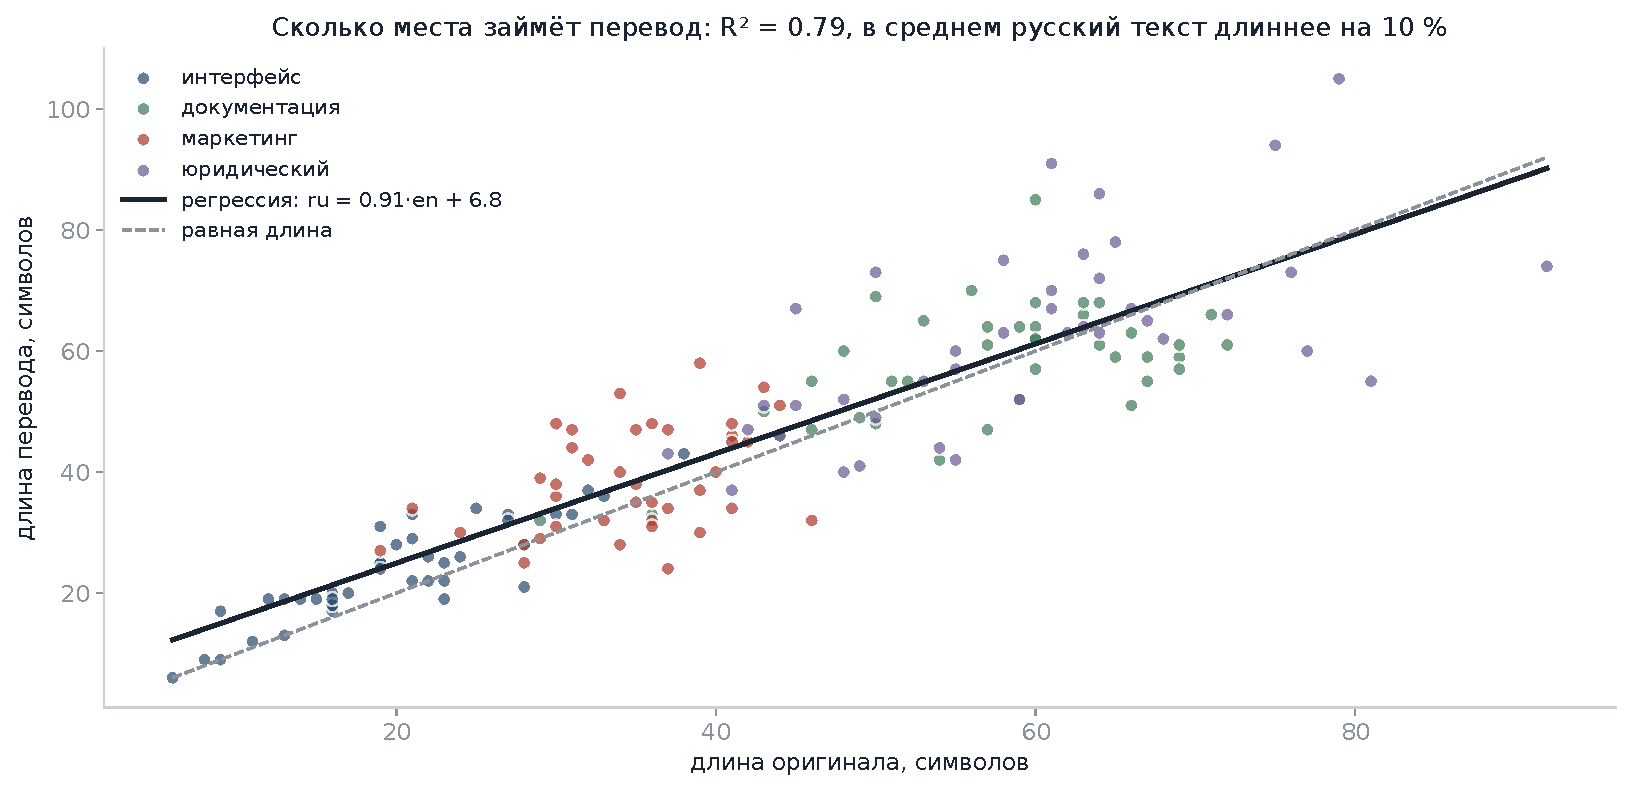
\includegraphics[width=.80\textwidth,height=4.05cm,keepaspectratio]{fig/regression.pdf}\par\raggedright{\small Каждая точка — сегмент: по горизонтали длина оригинала, по вертикали длина перевода. Рисунок помогает рассмотреть зависимость и необычные наблюдения.}
\врезка{График рассматривают до интерпретации коэффициентов: связь может быть нелинейной или различаться по группам.}
\end{frame}

\begin{frame}{Корреляция Пирсона}
\color{ink}
{\small \[\displaystyle r=\frac{\sum_i(x_i-\overline x)(y_i-\overline y)}{\sqrt{\sum_i(x_i-\overline x)^2\sum_i(y_i-\overline y)^2}}\]
\par\vspace{0.6em}Коэффициент измеряет линейную связь двух непостоянных признаков и лежит от −1 до 1. Знак показывает направление, модуль — силу линейной связи.}
\врезка{r = 0 означает отсутствие линейной корреляции; нелинейная зависимость при этом возможна. Корреляция не доказывает причинность.}
\end{frame}

\begin{frame}{Ранговая корреляция}
\color{ink}
{\small Ранговая корреляция сопоставляет порядок объектов по двум показателям. Она удобна, если важна согласованность ранжирования, а не линейная зависимость значений.
\par\vspace{0.6em}Например, BLEU и chrF могут по-разному оценивать величину сходства, но сходным образом упорядочивать сегменты.}
\врезка{Согласованность двух метрик не означает согласованности с человеческой оценкой. Для неё нужен отдельный набор разметки.}
\end{frame}

\begin{frame}{Интерполяция и экстраполяция}
\color{ink}
{\small Интерполяция оценивает значение внутри области наблюдений, экстраполяция — за её пределами. При прогнозе длины перевода область задаётся длинами и типами обучающих сегментов.
\par\vspace{0.6em}Для коротких кнопок модель, обученная только на длинных абзацах, может давать ненадёжный прогноз.}
\врезка{Обе операции применимы к числовым признакам текстов. Однако смысловую близость строк нельзя свести к промежуточной точке на прямой.}
\end{frame}

\begin{frame}{Нейронная сеть: место в обработке текста}
\color{ink}
{\small Нейронная сеть получает числовые представления и последовательно их преобразует. Выход зависит от задачи: метки классов, вектор сегмента или распределение токенов.
\par\vspace{0.6em}В локализации часто используют уже обученную сеть, а качество её результата проверяют на своих материалах.}
\end{frame}

\begin{frame}{Искусственный нейрон}
\color{ink}
\centering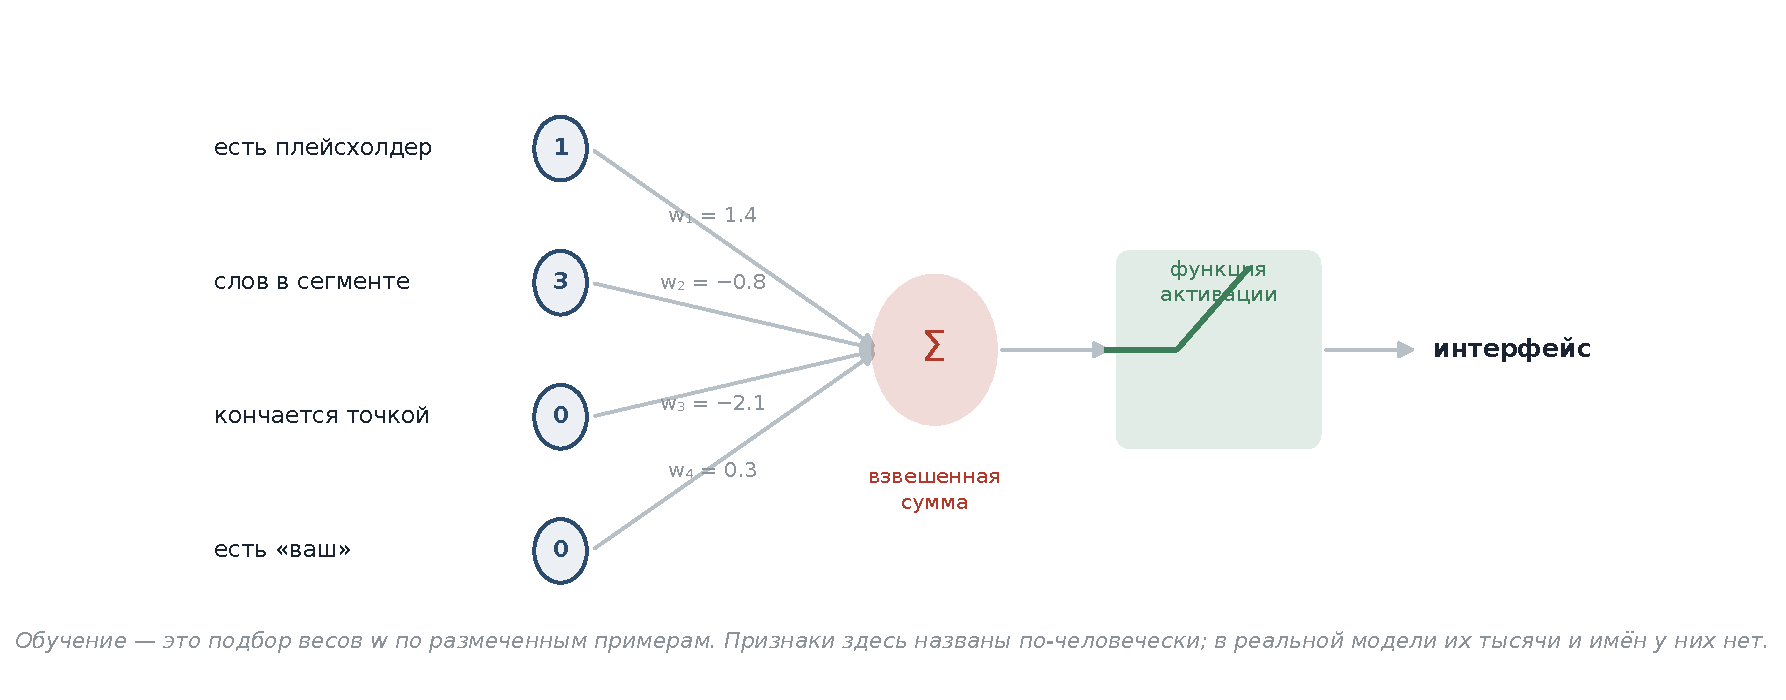
\includegraphics[width=.80\textwidth,height=4.05cm,keepaspectratio]{fig/neuron.pdf}\par\raggedright{\small Нейрон вычисляет $h=\varphi(\sum_jw_jx_j+b)$. Веса определяют вклад признаков, смещение — сдвиг суммы, активация — её преобразование.}
\врезка{Параметры подбирают по функции потерь. Для сети из нескольких слоёв градиенты вычисляют обратным распространением ошибки.}
\end{frame}

\begin{frame}{Функции активации}
\color{ink}
{\small \[\displaystyle \operatorname{ReLU}(z)=\max(0,z),\qquad\sigma(z)=\frac1{1+e^{-z}}\]
\par\vspace{0.6em}ReLU используется во многих скрытых слоях. Сигмоида подходит, например, для вероятности в бинарной классификации и для управляющих элементов рекуррентных сетей.}
\врезка{В трансформерах встречаются GELU и другие активации. Единой функции для всех архитектур нет.}
\end{frame}

\begin{frame}{Обучение сети}
\color{ink}
{\small \[\displaystyle \theta\leftarrow\theta-\eta\nabla_\theta L\]
\par\vspace{0.6em}Функция потерь L задаёт критерий ошибки. Градиент показывает направление её локального роста по параметрам; шаг с минусом направлен на уменьшение потерь.}
\врезка{Потери на обучении и качество на новых данных проверяют отдельно. Снижение одного показателя не гарантирует улучшения другого.}
\end{frame}

\begin{frame}{Токенизация в языковых моделях}
\color{ink}
{\small Подсловная токенизация разбивает строку на элементы конечного словаря. Частое слово может стать одним токеном, редкое — несколькими.
\par\vspace{0.6em}Границы токенов не обязаны совпадать с морфемами. Число токенов русской строки зависит от конкретного токенизатора.}
\врезка{Нельзя заранее назначить универсальный коэффициент «русский текст всегда вдвое длиннее английского». Проверяют реальные строки и выбранную модель.}
\end{frame}

\begin{frame}{Токены, эмбеддинги и позиции}
\color{ink}
\begin{center}\begin{tikzpicture}[>=Stealth,box/.style={draw=navy!40,fill=paper,align=center,text width=2.45cm,minimum height=1.35cm,font=\small,inner sep=5pt}]\node[box] (n0) at (0.0,0) {Текст и\\токенизация};
\node[box] (n1) at (3.15,0) {Коды\\токенов};
\node[box] (n2) at (6.3,0) {Векторы\\и позиции};
\node[box] (n3) at (9.45,0) {Векторы\\с контекстом};
\draw[->,thick,navy] (n0) -- (n1);
\draw[->,thick,navy] (n1) -- (n2);
\draw[->,thick,navy] (n2) -- (n3);\end{tikzpicture}\end{center}{\small Слои трансформера изменяют вектор каждой позиции с учётом доступного контекста.}
\врезка{Одинаковый токен может получить разные контекстные представления в разных предложениях. Начальный вектор выбирается из общей таблицы.}
\end{frame}

\begin{frame}{Механизм внимания}
\color{ink}
{\small Внимание вычисляет веса взаимодействия между позициями и строит взвешенную сумму их представлений.
\par\vspace{0.6em}\[\displaystyle \operatorname{Attention}(Q,K,V)=\operatorname{softmax}\!\left(\frac{QK^\top}{\sqrt{d_k}}\right)V\]}
\врезка{Q, K, V — обучаемые проекции входных векторов; $d_k$ — размерность ключа. Softmax превращает оценки связей в нормированные веса.}
\end{frame}

\begin{frame}{Доступ к контексту}
\color{ink}
\begin{columns}[T,onlytextwidth]\column{.45\textwidth}\centering\begin{tikzpicture}[x=.65cm,y=.65cm]\filldraw[fill=navy!55,draw=white] (0,0) rectangle ++(1,-1);\filldraw[fill=paper,draw=white] (1,0) rectangle ++(1,-1);\filldraw[fill=paper,draw=white] (2,0) rectangle ++(1,-1);\filldraw[fill=paper,draw=white] (3,0) rectangle ++(1,-1);\filldraw[fill=paper,draw=white] (4,0) rectangle ++(1,-1);\filldraw[fill=navy!55,draw=white] (0,-1) rectangle ++(1,-1);\filldraw[fill=navy!55,draw=white] (1,-1) rectangle ++(1,-1);\filldraw[fill=paper,draw=white] (2,-1) rectangle ++(1,-1);\filldraw[fill=paper,draw=white] (3,-1) rectangle ++(1,-1);\filldraw[fill=paper,draw=white] (4,-1) rectangle ++(1,-1);\filldraw[fill=navy!55,draw=white] (0,-2) rectangle ++(1,-1);\filldraw[fill=navy!55,draw=white] (1,-2) rectangle ++(1,-1);\filldraw[fill=navy!55,draw=white] (2,-2) rectangle ++(1,-1);\filldraw[fill=paper,draw=white] (3,-2) rectangle ++(1,-1);\filldraw[fill=paper,draw=white] (4,-2) rectangle ++(1,-1);\filldraw[fill=navy!55,draw=white] (0,-3) rectangle ++(1,-1);\filldraw[fill=navy!55,draw=white] (1,-3) rectangle ++(1,-1);\filldraw[fill=navy!55,draw=white] (2,-3) rectangle ++(1,-1);\filldraw[fill=navy!55,draw=white] (3,-3) rectangle ++(1,-1);\filldraw[fill=paper,draw=white] (4,-3) rectangle ++(1,-1);\filldraw[fill=navy!55,draw=white] (0,-4) rectangle ++(1,-1);\filldraw[fill=navy!55,draw=white] (1,-4) rectangle ++(1,-1);\filldraw[fill=navy!55,draw=white] (2,-4) rectangle ++(1,-1);\filldraw[fill=navy!55,draw=white] (3,-4) rectangle ++(1,-1);\filldraw[fill=navy!55,draw=white] (4,-4) rectangle ++(1,-1);
\node[font=\small,above] at (2.5,.3) {Позиции контекста};
\node[font=\scriptsize,rotate=90] at (-.5,-2.5) {Текущая позиция};\end{tikzpicture}
\column{.49\textwidth}{\small Синие клетки — доступные позиции. Серые — будущие позиции, закрытые маской.
\par\vspace{.6em}При предсказании следующего токена модель использует текущий префикс. В двунаправленном кодировщике ограничение другое.}\end{columns}
\врезка{Это схема доступности, а не измеренные веса внимания. Маска не гарантирует правильного использования доступного контекста.}
\end{frame}

\begin{frame}{Стоимость полного внимания}
\color{ink}
{\small В полном самовнимании оцениваются связи между парами позиций. Для последовательности длины n матрица оценок содержит n² элементов.
\par\vspace{0.6em}Удвоение длины увеличивает размер этой матрицы в четыре раза. Стоимость всей модели зависит также от остальных слоёв и реализации.}
\врезка{Это свойство полного внимания. Разреженные и иные варианты могут иметь другую зависимость от длины.}
\end{frame}

\begin{frame}{GPT: авторегрессионный трансформер}
\color{ink}
{\small Семейство GPT использует декодерную архитектуру: по предыдущим токенам оценивается распределение следующего. Название раскрывается как Generative Pre-trained Transformer.
\par\vspace{0.6em}Предобучение по продолжениям текста создаёт общую основу. Дополнительное обучение может настраивать выполнение инструкций и другие свойства.}
\врезка{Описание архитектуры не является гарантией достоверности ответа. Сохранность смысла проверяют по оригиналу и контексту.}
\end{frame}

\begin{frame}{Предобучение и дообучение}
\color{ink}
\begin{columns}[T,onlytextwidth]\column{0.47\textwidth}{\small \textbf{Предобучение.} Получение общих представлений и закономерностей на большом наборе данных.
\par\vspace{0.6em}Задача может состоять в предсказании следующего токена или восстановлении скрытых элементов.}
\column{0.47\textwidth}{\small \textbf{Дообучение.} Продолжение обучения для нужного домена, формата или способа ответа.
\par\vspace{0.6em}Время и необходимый объём данных зависят от размера модели и постановки задачи.}\end{columns}
\end{frame}

\begin{frame}{Применение модели к переводу}
\color{ink}
{\small Выбрать сегменты, характерные для проекта. Получить перевод готовой моделью. Сопоставить его с оригиналом, терминологией и техническими ограничениями.
\par\vspace{0.6em}Сравнивать версии модели при одинаковых условиях. Результат усреднения дополнить разбором критических ошибок.}
\end{frame}

\begin{frame}{Методы и лабораторные работы}
\color{ink}
{\small\renewcommand{\arraystretch}{1.15}\begin{tabular}{@{}Л{0.29} Л{0.44} Л{0.19}@{}}\toprule
Задача & Средства & Практика\\\midrule
Тип контента & TF-IDF и классификатор & Л.р. № 1\\[0.15em]
Подсказка из памяти & Левенштейн, LSA, эмбеддинги & Л.р. № 2\\[0.15em]
Качество перевода & Метрики, правила, ручная разметка & Л.р. № 3\\[0.15em]
Генерация & N-граммная модель, GRU & Л.р. № 4\\[0.15em]\bottomrule\end{tabular}}
\end{frame}

\begin{frame}{Вопросы для обсуждения}
\color{ink}
{\small Как отличить необычный, но корректный сегмент от ошибочного?
\par\vspace{0.6em}Почему высокая корреляция метрик не доказывает их пригодность для приёмки?
\par\vspace{0.6em}Что изменится, если удалить пунктуацию перед проверкой подстановочных полей?
\par\vspace{0.6em}Какие различия между предобучением и применением модели важны для проекта?}
\end{frame}

\begin{frame}{Источники}
\color{ink}
{\small \href{https://arxiv.org/abs/1706.03762}{Vaswani et al. (2017): Attention Is All You Need}.
\par\vspace{0.6em}\href{https://web.stanford.edu/~jurafsky/slp3/}{Jurafsky, Martin: Speech and Language Processing}.
\par\vspace{0.6em}\href{https://scikit-learn.org/stable/user_guide.html}{scikit-learn: анализ данных и оценка моделей}.
\par\vspace{0.6em}Учебный корпус и его описание: папка data; подготовка данных и оценка: лабораторные курса.}
\end{frame}

\end{document}
